\chapter{Control-Flow-Driven Verification}\label{ch:cfg}
The memory usage analysis approach presented in this chapter
provides a Floyd-style methodology featuring annotations on specific instructions.
It is designed for the proving of memory preservation%
\index{memory!preservation}
over individual assembly functions.
That property ensures that only documented regions of memory are modified;%
\index{memory!region}
anything outside of those regions remains unchanged.

This control-flow-driven verification
can be applied to functions with loops and subcalls,
including directly-recursive calls.
It can be used to prove the absence of common memory-related issues,
such as buffer and stack overflows. In cases where overflow may occur,
the methodology helps extract the assumptions required to prevent that.
For efficiency, it selects the annotation locations,
called \emph{cutpoints},%
\index{cutpoint}
such that every path through the program
is symbolically executed only once.%
\index{symbolic execution}

An overview of the methodology's steps can be seen in \cref{se:cfg_overview},
with formal definitions of the needed constructs presented in \cref{se:cfg_defs}.
Following that, \cref{se:cfg_composition} describes how the method uses composition
on the function level and within function bodies.
Two examples providing a brief demonstration of the methodology
can be found in \cref{se:cfg_examples}, while a real-world application
to the HermitCore unikernel library \autocite{lankes2016hermitcore}
is presented in \cref{se:cfg_application}.
Our observations regarding usage of the methodology on that case study
are given in \cref{se:usability}.

My three main contributions to the memory preservation work presented here were:
\begin{enumerate*}
  \item the development of a tool for producing proof skeletons
  for memory preservation, interfacing with the analysis tool
  \texttt{angr} (\cref{se:cfg_overview});
  \item the development of structured proof strategies
  to flesh out and verify those skeleton proofs,
  along with the development of guidelines
  for invariants that provide for
  function-level composition (\cref{se:cfg_composition});
  and
  \item the application of the methodology to functions in
  \cref{sse:pow2_example,se:cfg_application}.
\end{enumerate*}

\section{Overview of Methodology}\label{se:cfg_overview}
The first step in the process of analysis for a function
is disassembly of an \arch\ binary containing it.
This is done using a modified version of the \lstinline|reassembly| analysis
\autocite{wang2017ramblr} of the binary analysis tool \texttt{angr} \autocite{shoshitaishvili2016state,wang2017angr}.%
\index{\texttt{angr}}
That modified version was provided by \textcite{roessle2019}
for generating assembly usable with their Isabelle parser.%
\index{\texttt{angr}!\texttt{reassembly}}
By building on \texttt{angr},
the work of abstracting from binary to \ac{cfg} is handled with minimal user input.

To achieve minimal symbolic execution, cutpoints%
\index{cutpoint}
are automatically selected by a Python package that relies on
\texttt{angr}'s \lstinline|CFGEmulated| control flow analysis.%
\index{\texttt{angr}!CFGEmulated}
The cutpoints are described in \cref{se:cfg_invariant}.
Basic starting predicates for those preconditions and postconditions%
\index{precondition}%
\index{postcondition}
as well as the cutpoints are generated,
but the bulk of the information must be added manually.
Larger-scale scalability is achieved by using function-level compositionality.
Even recursive functions are supported, albeit with difficulty.%
\index{recursion}

The process that selects cutpoints%
\index{cutpoint}
also generates skeleton memory preservation theories for every function analyzed.
The theory files can then be opened in the theorem prover Isabelle
and the assembly loaded using the parser of \textcite{roessle2019}.
Once that is done, a user can flesh out the invariants (\cref{se:cfg_invariant})
and add the necessary sets of memory regions that the functions write to
in order to complete the proofs of memory preservation.
Defining the necessary invariants for functions with complex control flow
is generally a hard task, but targeting a property such as memory preservation
does reduce the amount of work required
as seen in \cref{se:cfg_examples,se:cfg_application}.
The work is still not trivial, however.

\begin{figure}
  \centering
  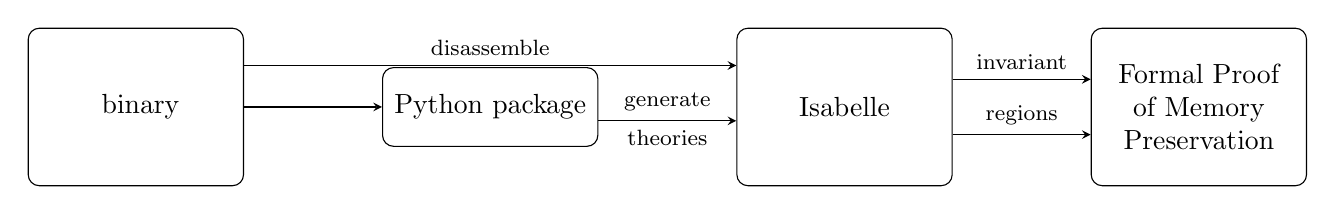
\begin{tikzpicture}[node distance=4.5cm, auto, ->, >=stealth, myblock/.style={
    draw,
    text width=2.5cm,
    text centered,
    rounded corners,
    minimum height=2cm
  }]
    \node[myblock] (binary) {\arch\ binary};
    \node[myblock, right of=binary, minimum height=1cm] (cfg) {Python package};
    \node[myblock, right of=cfg] (isa) {Isabelle};
    \node[myblock, right of=isa] (mem) {Formal Proof of Memory Preservation};

    \draw[transform canvas={yshift=1.5em}] (binary) -- node[above] {\footnotesize disassemble} (isa);
    \draw (binary) -- (cfg);
    \draw[transform canvas={yshift=-.5em}] (cfg) -- node[above] {\footnotesize generate} node[below] {\footnotesize theories}(isa);
    \draw[transform canvas={yshift=1em}] (isa) -- node[above] {\footnotesize invariant} (mem);
    \draw[transform canvas={yshift=-1em}] (isa) -- node[above] {\footnotesize regions} (mem);
  \end{tikzpicture}
  \caption{Overview of control-flow-driven memory preservation verification}\label{fig:cfg_overview}
\end{figure}

\section{Formal Definitions}\label{se:cfg_defs}
A formal definition of memory preservation requires a formal basis to work with,
and that basis is the machine model from \cref{se:machine_model}.

\subsection{Symbolic Execution for \acs*{cfg}-Driven Verification}\label{cfg_symb_exec}
While \cref{ch:symbolic_execution} provided a general overview of symbolic execution,
this chapter requires a more specific look.
The step function for this methodology takes the form
$\step:S\rightarrow(S\mid\bot_E)$.%
\nomenclature{$S$}{Type representing program state; an Isabelle record}%
\nomenclature{$\bot_E$}{Indicates exceptional state}
It takes the current state~$\sigma$ to execute from
and returns the state~$\sigma'$ after execution of the current instruction,
which is extracted from the current state based on the value of the instruction pointer
\inlineasm{rip}.
If some sort of exception, such as a divide by zero, occurs,
the function returns~$\bot_E$ instead.

From the machine model, we manually derived a run function%
\index{symbolic execution!run function}
$\run:(S\rightarrow\mathbb{B})\times S\rightarrow(S\mid\bot_E\mid\infloop)$.
This partial function takes as input a state predicate~$H$ and a state~$\sigma$,%
\index{state!predicate}
producing a state~$\sigma'$ on successful completion.
Predicate~$H$ denotes a \emph{halting condition},%
\index{symbolic execution!halting condition}
which typically instructs the run function to stop
at a certain instruction address, such as that following a \inlineasm{ret}.
The run function executes $\step$ until~$H$, applied to the current state,
is true. Whenever an exception occurs, it stops and returns~$\bot_E$.
If the execution were to continue forever
without an exception or reaching the halting condition
(as would happen with an infinite loop), the function returns $\bot_\var{NT}$.
Formally, this is achieved by a standard \ac{lfp} construction.

\subsection{Hoare Triples for Memory Preservation}
Unlike the usual formulation of
Hoare logic \autocite{hoare1969axiomatic,myreen2007hoare},%
\index{Hoare!logic}
Hoare triples for this work take one of the aforementioned halting conditions%
\index{Hoare!triple}
as their middle input rather than a program statement.
The result is that the program statement,
the block of instructions to execute, is characterized by the addresses of its initial
and ending instructions, defined in~$P$ and~$H$, rather than via specific syntax.
Thus, we have the following definition:
\begin{definition}[Hoare triple for memory preservation]\label{def:htriple}
  $\htriple{P}H{Q}$
  denotes that, for any initial state that satisfies the precondition~$P$
  and results in symbolic execution to the halting condition~$H$ terminating,
  the resultant state will be non-exceptional and satisfy postcondition~$Q$.

  This is formally expressed as:
  \begin{equation}
  \htriple{P}H{Q}\equiv\forall\sigma\cdot
  P(\sigma)\wedge\sigma'\neq\infloop\longrightarrow
  \sigma'\neq\bot_E\wedge Q(\sigma'),
  \end{equation}
  where $\sigma'=\run(H,\sigma)$.
\end{definition}

\subsection{Floyd Invariant Foundation}\label{se:cfg_invariant}
Loops pose a significant problem when using symbolic execution to analyze code.%
\index{loop}
One of the major issues is that they result in significant path explosion.%
\index{loop!path explosion}
While there are methodologies to reduce the number of paths to execute
when using loops \autocite{saxena2009lese,obdrzalek2011efficient},
those methods are not currently formally verified
and therefore not usable within Isabelle/HOL.
Additionally, deciding the loop condition on a symbolic state
may involve non-determinism (such as an event loop dependent on user input to exit),%
\index{non-determinism}
which can cause infinite execution.

Breaking up symbolic execution of loops is one method of resolving those issues.
With the right annotations,
it is possible to only need to symbolically execute one iteration per loop.
This eliminates the above-mentioned loop issues.
That breaking up of loops can be accomplished using a control-flow-based approach
akin to Floyd verification \autocite{floyd1967assigning}.%
\index{Floyd!verification}
A state predicate that can be shown to hold for every iteration of a loop
at some instruction within that loop will function as a \emph{loop invariant},%
\index{loop!invariant}
symbolically characterizing the loop's behavior.
This can be combined with a general methodology of structured preconditions and postconditions over annotated locations.
If that methodology can show that the state at one such location
satisfying the location's annotation will lead to any succeeding annotated locations
also having states that satisfy their annotations,
a Hoare triple as defined in \cref{def:htriple}
can be inferred for the program as a whole (\cref{thm:floyd_hoare}).

More formally, the \emph{Floyd invariant}%
\index{Floyd!invariant}
for a function is a partial function that takes the form
$I:L\rightharpoonup(S\rightarrow\mathbb{B})$.%
\nomenclature{$L$}{Type of instruction addresses in a program; a 64-bit word}%
\nomenclature{$\mathbb{B}$}{Type of boolean values, True and False}
This function maps from instruction addresses with invariants
to the corresponding state predicate that is the invariant.
As a technical detail, some function proofs require additional arguments to $I$
that represent the arguments passed to the function.
\begin{definition}[Floyd invariant]\label{def:floyd_inv}
  A Floyd invariant~$I$ \emph{holds} if and only if, for any state~$\sigma$,
  \begin{equation}
    I(\loc\sigma)(\sigma)\longrightarrow
    \sigma'\neq\bot_E\wedge(\sigma'=\infloop\vee I(\loc\sigma')(\sigma')),
  \end{equation}
  where
  $\sigma'=\run((\lambda\sigma\cdot I(\loc\sigma)(\sigma)\neq\bot),\sigma)$%
  \nomenclature{$\bot$}{Used here to represent an empty value,
    such as the result of calling a partial function with a value it does not have an actual result for or in general the \texttt{None} value of an optional type}
  and $\loc\sigma$ is the current program location,
  stored in \inlineasm{rip} on \arch\ systems.
\end{definition}
In words, if the Floyd invariant holds on the current state,
then running to the next annotated location will not produce an exception.
If that run terminates, then the state it produces
will also satisfy the Floyd invariant.

The following theorem states that a Floyd invariant
can be used to prove properties over its corresponding program or function
as a whole:
\begin{theorem}[Floyd and Hoare]\label{thm:floyd_hoare}
  Assume that Floyd invariant~$I$ holds and provides annotations for locations~$l_0$ and~$l_f$ (the initial and final location).
  Let halting condition~$H$ stop at location~$l_f$;%
  \index{halting condition}
  that is, $H(\sigma)\longrightarrow\loc\sigma=l_f$.
  Then $\htriple{I(l_0)}{H}{I(l_f)}$.
\end{theorem}
\begin{proof}
  Remember from \cref{def:htriple} that
  \begin{equation*}
    \htriple{P}H{Q}\equiv\forall\sigma\cdot
    P(\sigma)\wedge\sigma'\neq\infloop\longrightarrow
    \sigma'\neq\bot_E\wedge Q(\sigma').
  \end{equation*}
  Though there could be any number of additional annotations between~$l_0$
  and~$l_f$, \textcite{floyd1967assigning} showed by induction
  that a Floyd invariant that holds starting from some initial condition
  to an intermediate annotation at~$l_1$ will also hold starting from that annotation.
  Thus, as~$I$ holds, we can substitute in~$I(l_0)(\sigma)$ for~$P(\sigma)$
  and~$I(l_f)(\sigma')$ for~$Q(\sigma')$ without issue,
  resulting in the following statement:
  \begin{equation*}
      I(l_0)(\sigma)\wedge\sigma'\neq\infloop\longrightarrow
      \sigma'\neq\bot_E\wedge I(l_f)(\sigma').
  \end{equation*}
  As we have already assumed that~$I$ holds,
  we can substitute in the right side of the implication from \cref{def:floyd_inv}
  to obtain
  \begin{equation*}
    \sigma'\neq\bot_E\wedge(\sigma'=\infloop\vee I(l_f)(\sigma'))\wedge
    \sigma'\neq\infloop\longrightarrow
    \sigma'\neq\bot_E\wedge I(l_f)(\sigma').
  \end{equation*}
  This then simplifies to
  \begin{equation*}
    \sigma'\neq\bot_E\wedge I(l_f)(\sigma')\longrightarrow
    \sigma'\neq\bot_E\wedge I(l_f)(\sigma'),
  \end{equation*}
  which is trivial.
\end{proof}
In essence, Floyd-style verification%
\index{Floyd!verification}
models a program as \iac{cfg} where each edge is an implication.

\subsection{Definition of Memory Preservation}\label{sse:mem_pres}
The formal definition of memory preservation%
\index{memory!preservation}
takes the form of a Hoare triple from \cref{def:htriple}.
Initially, there must be some predicate~$P$ that characterizes the initial state,
at a minimum by setting the instruction pointer
to the first instruction of the relevant function body.
In addition, there is some set of memory regions~$M$
that the function is allowed to write to.
$M$ includes the stack frame and any utilized data sections from the source binary,
as well as whatever heap memory was supplied or allocated, if any.
Memory preservation formulates that any byte not within any of the regions in~$M$
has to remain unchanged throughout the execution of that function.
The notation for this formulation is shown below.
\begin{definition}[Memory preservation]\label{mem_pres_hoare}
  Let~$M$ be a set of memory regions, let~$P$ be a precondition,
  and let~$H$ denote a halting condition.
  A piece of assembly demonstrates \emph{memory preservation} if and only if,
  for any address~$a$ and byte value~$v_0$, the following implication holds:
  \begin{equation}
  (\forall r\in M\cdot r\separate\region{a}1)\longrightarrow\htriple{P\wedge \readmem{a}1=v_0}H{Q\wedge\readmem{a}1=v_0}
  \end{equation}
\end{definition}
This definition states that, for every byte in memory outside of the memory region set,
the following property holds:
\begin{enumerate}
  \item if you start the current program fragment from a state that both satisfies
  the specified precondition and assumes that each byte has some value, then;
  \item if you execute that program fragment to the specified halting condition, then;
  \item you will end up with a state that satisfies the specified postcondition
  and retains the same value for all of those bytes outside the memory regions.
\end{enumerate}

\section{Composition}\label{se:cfg_composition}
As stated above, composition is used here for scalability.%
\index{composition}
On the function call level, compositionality ensures that,
when a function is called,
a successful verification effort over that function can be reused
if preexisting or developed later if need be.
Taking this approach also allows minimizing symbolic execution
even in non-loop situations, a form of internal compositionality.

\subsection{Intra-Function}
Consider the following pseudocode,
which sequentially executes an if-statement and some program~$P$:
\begin{lstlisting}[
  escapechar=|,
  gobble=2,
  caption=Simple pseudocode,
  label=compositional_pseudocode
]
  if |$b$| then |$x$| else |$y$|; |$P$|
\end{lstlisting}
The assembly corresponding to this code can be verified using symbolic execution.
If executed in full, the symbolic execution engine
would require first considering the case where~$b$ is true,
executing~$x$ and subsequently symbolically executing program~$P$.
It would then consider the case where~$b$ is false, executing~$y$ followed by~$P$.
Program~$P$ would thus be symbolically executed twice.
This repetition can be avoided
by placing a cutpoint at the start of each block where control flow converges,%
\index{cutpoint}
resulting in all instructions being symbolically executed only once each.
Each cutpoint, however, requires a state predicate contained in a Floyd invariant.

Reasoning about composition with the Hoare triples specific to this chapter
requires a bit of work,
as standard composition does not apply to Hoare triples
that use halting conditions.%
\index{symbolic execution!halting condition}
Doing so is still possible, however.
\begin{theorem}[Composition rule]\label{thm:comp}
  Halting Hoare triples are compositional
  with respect to stronger halting conditions:
  \begin{prooftree}
    \AxiomC{$\htriple{P}H{Q}$}
    \AxiomC{$\htriple{Q}{H'}{R}$}
    \AxiomC{$\forall\sigma\cdot H'(\sigma) \longrightarrow H(\sigma)$}
    \TrinaryInfC{$\htriple{P}{H'}{R}$}
  \end{prooftree}
\end{theorem}
\begin{proof}
  Consider a symbolic run that executes until halting condition~$H'$.
  It is possible to break this run into two parts
  by first running until a halting condition~$H$ and then until~$H'$.
  This requires that~$H'$ is \emph{stronger} than~$H$; that is,~$H'$ implies~$H$.
  Doing so ensures that the run first stops at~$H$ before it stops at~$H'$
  (as it is possible for $H$ to hold when $H'$ does not,
  but not the other way around).
\end{proof}
\begin{example}
  Now consider the block of assembly that could be generated for
  \cref{compositional_pseudocode}.
  Let~$l_f$ denote the final location of the block
  while~$l_P$ denotes the initial location of program~$P$.
  \Cref{thm:comp} can be used by instantiating~$H$ to halt
  at either location~$l_f$ or~$l_P$ and instantiating~$H'$ to halt at~$l_f$.
  As long as programs~$x$ and~$y$ do not contain \lstinline[style=C]|goto|s
  or some other instruction that violates expected control flow,
  condition~$H$ will ultimately be equivalent to just halting at~$l_P$.
  As~$H'$ is stronger than~$H$, compositionality is possible.
\end{example}

\subsection{Function Calls}\label{cfg:function_calls}
Generally, compositionality over function calls requires proving
that the stack pointer, after execution of a return,%
\index{stack!pointer}
has the same value it did before the corresponding function call.
Practically, this means proving that the body of the function
results in $\mathrsp=\rspo+8$.
This can be proven even for functions with optimized tail calls
that just swap the final \inlineasm{call}+\inlineasm{ret}
combo for a jump as long as the body of the called function
is treated as part of the callee.
\begin{example}
  Consider a function~$f$ starting in a text section at location~$l_0$.
  The function is called from a different text section
  by the instruction \inlineasm{call f} at location~$l_\var{call}$.
  This means the return address for the call is $l_\var{call}+5$.%
  \footnote{the \texttt{call} instruction is five bytes long}
  After execution of \inlineasm{call f}, the program will be at location~$l_0$
  and the stack pointer, \inlineasm{rsp}, will have some value $\rspo$.
  In order to apply compositionality to function calls,
  the pre- and postcondition have to meet the following requirements.
  First, the precondition must imply that the return address is pushed on the stack
  (a task performed by \lstinline{call}):
  $\readmem{\rspo}{8}=l_\var{call}+5\wedge\mathrsp=\rspo$.
  Second, the postcondition must imply that after \lstinline{ret},
  the net effect of the function body
  is that the stack pointer has been incremented by 8:
  $\mathrsp=\rspo+8\wedge\loc=l_\var{call}+5$.
  Note that \lstinline{call} itself decrements the stack pointer by~8,
  so this implies the net effect, from the point of view of the caller,
  is that the stack pointer is unchanged.
  The postcondition must also show
  that the location has been set back to the return address, $l_\var{call}+5$.
\end{example}
Besides the stack pointer, modern calling conventions have other \emph{callee-saved}%
\index{register!callee-saved}
registers, such as \lstinline{rbp} and \lstinline{r12-r15}.
It is generally assumed that the net effect of a function call
does not touch these registers.
Consider a situation in which \lstinline{rbp} contains an address,
which will be used as the target of a write after a function call.
In order to prove memory preservation, \lstinline{rbp} must be shown to be preserved.
Generally, this is easy to prove
by strengthening the pre- and postcondition with a conjunct $\mathrbp=\rbpo$.
The proof is generally not complicated,
as these callee-saved registers are pushed onto the stack
at the beginning of functions that use them and popped off at the end.

In many cases, users of a verification methodology over functions
will encounter calls to functions that are not included in the verification effort.
These may be system calls or simply functions not currently under consideration
due to unsupported features or lack of time.
External functions are simply assumed to have correct behavior
and are thus left out of the existing analysis,
leaving those functions in the \ac{tcb}.
One issue that may occur is a desired function
making an optimized tail call to an external function,
which cannot be treated as part of the callee and prevents verification.
One possible solution, used in the next chapter,
is to revert the jump to \inlineasm{call}+\inlineasm{ret}.
As the underlying function is assumed to be correct,
this will result in the proper \inlineasm{rsp} restoration.

\section{Examples}\label{se:cfg_examples}
The following sections present some basic explanation
of the procedure used in this chapter via two simple functions.
The first, in \cref{sse:pow2_example}, is a non-recursive function that features a loop.
The second, in \cref{sse:factorial_example}, gives an example of a recursive function
and shows why those are difficult to reason about.

\subsection{Non-recursive Loop Example: \texttt{pow2}}\label{sse:pow2_example}
This simple loop-based function, shown in \cref{lst:pow2},
raises two to the power of its argument.
The assembly code was obtained by compiling a C program containing the function
with \ac{gcc} 7.2.0
and disassembling it using the modified \lstinline|reassembly| analysis
mentioned in \cref{se:cfg_overview}. The input is stored in \lstinline{edi}.
\begin{lstlisting}[
  style=C,
  gobble=2,
  float=*,
  caption=\texttt{pow2} in C,
  label=lst:pow2
]
  unsigned long pow2(unsigned exponent) {
      unsigned long a = 1;

      for (unsigned i = 0; i < exponent; ++i) {
          a += a;
      }

      return a;
  }
\end{lstlisting}
\begin{lstlisting}[
  style=x64,
  gobble=2,
  float=*,
  caption=\texttt{pow2} in \arch\ assembly,
  label=lst:pow2a,
  firstnumber=0
]
  pow2:
      push rbp # Size:1
      mov  rbp, rsp # Size:3
      mov  dword ptr [rbp - 0x14], edi # Size:3
      mov  qword ptr [rbp - 8], 1 # Size:8
      mov  dword ptr [rbp - 0xc], 0 # Size:7
      jmp  .label_10 # Size:2
  .label_11:
      shl  qword ptr [rbp - 8], 1 # Size:4
      add  dword ptr [rbp - 0xc], 1 # Size:4
  .label_10:
      mov  eax, dword ptr [rbp - 0xc] # Size:3
      cmp  eax, dword ptr [rbp - 0x14] # Size:3
      jb   .label_11 # Size:2
      mov  rax, qword ptr [rbp - 8] # Size:4
      pop  rbp # Size:1
      ret  # Size:1
\end{lstlisting}
The function uses memory in five places, all on the stack.
These are expressed relative to the original value of the stack pointer $\rspo$:
\begin{enumerate*}%[label=\alph*.)]
  \item the caller's \lstinline|rbp| at $\mathrbp=\rspo-8$ (eight bytes);
  \item the argument to the function at $\mathrbp-\mathtt{0x14}$ (four bytes);
  \item the accumulation variable and return value at $\mathrbp-8$ (eight bytes);
  \item the counter variable at $\mathrbp-\mathtt{0xc}$ (four bytes);
  \item and the address of the location to return to at $\rspo$.
\end{enumerate*}
The memory region for this function is thus $r_s=\region{\rspo-28}{36}$.
Assigning region~$r_s$ with ID~$i_s$
and the untouched region $\region{a}{1}$ with ID~$i_a$,
parent relationships can then be established as shown below:
\begin{align*}
  & \parent{\region{\rspo}8}{i_s}{r_s} && \parent{\region{\rspo-20}4}{i_s}{r_s} \\
  & \parent{\region{\rspo-8}8}{i_s}{r_s} && \parent{\region{\rspo-28}4}{i_s}{r_s} \\
  & \parent{\region{\rspo-16}8}{i_s}{r_s} && \parent{\region{a}1}{i_a}{\region{a}1}
\end{align*}

For the memory preservation proof of this function, we chose to associate annotations
at the start of the function, an instruction that broke the loop,
and the return address of the function
(a logical variable, as the caller of the function is unspecified for this proof).
\Cref{fig:pow2cfg} shows the Floyd invariant in \ac{cfg} form for this function.
The invariant carries through the preservation of memory,
showing that region $\region{a}{1}$ maintains its value throughout.
The equalities over \inlineasm{rbp} and \inlineasm{rsp}
are used by the memory region reasoner.
For compositional purposes, as described in \cref{se:cfg_composition},
the function is also shown to preserve the value of the stack pointer.
\begin{figure}
  \centering
  \begin{tikzpicture}[>=stealth]
    \graph[math nodes, grow down=2.2cm]{
      "1:\begin{array}{l}
        \readmem{a}{1}=v_0\wedge\mathrsp=\rspo\wedge{} \\
        \readmem{\rspo}{8}=\retaddr
      \end{array}" ->[
        align=left,
        "$\mathrsp\coloneqq\mathrsp-8$\\
        $\mathrbp\coloneqq\mathrsp$"
      ] b/"12:\begin{array}{l}
        \readmem{a}{1}=v_0\wedge~\\
        \mathrbp=\mathrsp=\rspo-8
      \end{array}" ->[
        "$\mathrsp\coloneqq\mathrsp+16$"
      ] "\retaddr:\readmem{a}{1}=v_0\wedge\mathrsp=\rspo+8";
      b ->[out=-16, in=16, looseness=3] b;
    };
  \end{tikzpicture}
  \caption{Floyd invariant for \texttt{pow2} in \acs*{cfg} form}\label{fig:pow2cfg}
\end{figure}
Given the parent regions presented above, the proof that the Floyd invariant holds
is executed automatically using the symbolic execution engine
described in \cref{ch:symbolic_execution}.

\subsection{Recursion: Factorial}\label{sse:factorial_example}
The factorial operation provides a simple example of recursion.%
\index{factorial}%
\index{recursion}
The basic definition of factorial is $n!=\prod_{i=1}^n i$.%
\nomenclature{$\prod$}{Product of a sequence of terms;
  multiplication equivalent of $\sum$}
This results in a number that is the product of the numbers from~$1$ to~$n$.
Expressed in recursive form, that definition is:
\begin{equation}
  n!=\begin{cases}
    n * (n - 1)! & \text{if }n > 0 \\
    1 & \text{if }n = 0
  \end{cases}
\end{equation}
The C equivalent of that function is shown in \cref{factorial-c}.
\begin{lstlisting}[
  style=C,
  gobble=2,
  float=*,
  caption=Factorial in C,
  label=factorial-c
]
  uint64_t factorial(uint8_t n) {
      if (n) {
          return n * factorial(n - 1);
      }
      return 1;
  }
\end{lstlisting}
The assembly snippet shown in \cref{lst:factasm} is again
the result of a function compiled with \ac{gcc} 7.2.0
and disassembled by the tweaked \lstinline|reassembly| analysis \autocite{wang2017ramblr}.
In this case, the function performs a recursive factorial calculation on the value~$n$
stored in~\lstinline|dil| (the lowest eight bits of~\lstinline|edi|/\lstinline|rdi|).
\begin{lstlisting}[
  style=x64,
  caption=\arch\ assembly of factorial example,
  label=lst:factasm,
  float,
  escapechar=|,
  firstnumber=0
]
  factorial:
      push  rbp|\label{factasm:precondition}|
      mov   rbp, rsp
      push  rbx
      sub   rsp, 0x18
      mov   eax, edi
      mov   byte ptr [rbp - 0x14], al
      cmp   byte ptr [rbp - 0x14], 0
      je    .label_12
      movzx ebx, byte ptr [rbp - 0x14]
      movzx eax, byte ptr [rbp - 0x14]
      sub   eax, 1
      movzx eax, al
      mov   edi, eax
      call  factorial
      imul  rax, rbx|\label{factasm:resume}|
      jmp   .label_13
  .label_12:
      mov   eax, 1
  .label_13:
      add   rsp, 0x18
      pop   rbx
      pop   rbp
      ret
\end{lstlisting}
It essentially consists of two loops,
one loop to perform storing the integers from~$n$ to 2 on the stack as the function
is called recursively
and the second to multiply all those values together as each call returns.

As with \lstinline|pow2|, the proof for this function relies on an~$\rspo$,
though in this case that value specifically refers to the value of \lstinline|rsp|
for the first/topmost call to the recursive function.
The memory locations operated on by this function
are similar to those of \lstinline|pow2|,
but the memory locations themselves cannot be directly offset
from~$\rspo$ due to the function's recursive nature.
\begin{figure*}
  \centering
  \begin{tikzpicture}[>=stealth]
    \graph[math nodes, grow down=3.5cm]{
      a/"1:\begin{array}{l}
        \readmem{a}{1}=v_0\wedge\mathdil\le n\wedge{} \\
        \mathrsp=\rspo-48*(n-\mathdil)\wedge{} \\
        (\mathdil\not=n\longrightarrow\mathrbx=\mathdil+1)\wedge{} \\
        \rbxpops(32,\rspo,n,\mathdil)\wedge{} \\
        \retsites(0,\rspo,n,\mathdil)
      \end{array}" ->[
        align=left,
        "$\begin{array}{l}
          \text{if }\mathdil = 0 \\
          \mathrsp\coloneqq\mathrsp+8
        \end{array}$"
      ] b/"15:\begin{array}{c}
        \readmem{a}{1}=v_0\wedge\mathrbx>0\wedge\mathrbx\le n\wedge{} \\
        \mathrsp=\rspo-48*(n-\mathrbx+1)+8\wedge{} \\
        \rbxpops(24,\rspo,n,\mathrbx-1)\wedge{} \\
        \retsites(8,\rspo,n,\mathrbx-1)
      \end{array}" ->[
        align=left,
        "$\begin{array}{l}
          \text{if }\mathrbx = n \\
          \mathrsp\coloneqq\mathrsp+48
        \end{array}$"
      ] "\retaddr:\readmem{a}{1}=v_0\wedge\mathrsp=\rspo+8";
      a ->[out=-17, in=17, swap, align=left, looseness=2,
        "$\text{if }\mathdil\neq 0$ \\
        $\mathrsp\coloneqq\mathrsp-48$ \\
        push \lstinline|rbx| \\
        $\mathrbx\coloneqq\mathdil$ \\
        $\mathrdi\coloneqq\mathdil-1$"
      ] a;
      b ->[out=-17, in=17, swap, align=left, looseness=2,
        "$\text{if }\mathrbx\neq n$ \\
        $\mathrsp\coloneqq\mathrsp+48$ \\
        pop \lstinline|rbx|"
      ] b;
    };
  \end{tikzpicture}
  \caption{Floyd invariant for factorial in \acs*{cfg} form}\label{fig:factcfg}
\end{figure*}
The set~$M$ of separated parent regions is characterized by the following assumptions:
\begin{subequations}
  \begin{align}
    \forall m\le n\cdot(i_m,\region{\rspo+48*m-(n*48)-40}{40}) &\in M \\
    \forall m\le n\cdot(i'_m,\region{\rspo+48*m-(n*48)}8) &\in M \\
    (i_a,\region{a}1) &\in M
  \end{align}
\end{subequations}
The first assumption models all stack frames of size~40.
The second models the parts of the stack where return addresses are pushed.
The parent relations are defined in a similar way.

The following functions assist in characterizing the stack frame
for any particular call in the recursive chain.
To start with, $\rbxpops$ characterizes the multiplicands currently stored on the stack
for any particular recursive call,
both in the initial recursing loop as well as in the second loop
as the recursive calls return.
The following functions, $\retaddress$ and $\retsites$,
establish that return address~15 is pushed
to the correct memory location for every call except the first.
For the first call, the topmost stack frame,
the initial return address must also be properly stored.
\begin{multline}
  \rbxpops(\var{offset},\rspo,n,x)\equiv \\
  \forall i\cdot n>x\wedge
    i<n-x-1\longrightarrow\readmem{\mathrsp+i*48+\var{offset}}{8}=i+1+\mathrbx
  \label{eq:rbxpops}
\end{multline}
\begin{multline}
  \retaddress(\var{rsp},\rspo,\var{offset},n,x,i)\equiv \\
  \text{if }\var{rsp}+(n-x-i)*48-\var{offset}=
  \rspo\text{ then }\retaddr \text{ else } 15
  \label{eq:ret_address}
\end{multline}
\begin{multline}
  \retsites(\var{offset},\rspo,n,x)\equiv \\
  \forall i\le n-x\cdot
    \readmem{\mathrsp+(n-x-i)*48-\var{offset}}{8}=
    \retaddress(\mathrsp,\rspo,\var{offset},n,x,i)
  \label{eq:retsites}
\end{multline}

The Floyd invariant for the factorial function is shown in
\cref{fig:factcfg,eq:rbxpops,eq:ret_address,eq:retsites}.
The first loop, from location~1 back to~1, goes deeper into recursion,
pushing values onto the stack until \inlineasm{dil} becomes~0.
As stated, $\rbxpops$ and $\retsites$ characterize the stack frame for every call,
ensuring that all necessary information is properly stored.
Once $\mathdil=0$, the function has executed its final recursion
and control reaches location~15.
The second loop then pops values of the stack until $n=\mathrbx$,
at which point there are no more recursive stack frames to pop
and the final result of the factorial operation can be returned.

A Hoare triple can now be derived from the the Floyd invariant.
This is done by instantiating variable~$n$ with \lstinline|dil|.
Doing so simplifies the precondition,
as initially, no values or return addresses are pushed
other than the upmost return address. The resulting Hoare triple becomes:
\begin{equation}
  \begin{array}{l}
    \{\readmem{a}{1}=v_0\wedge\mathrsp=\rspo\wedge\readmem{\rspo}{8}=\retaddr\} \\
    H \\
    \{\readmem{a}{1}=v_0\wedge\mathrsp=\rspo+8\wedge\loc=\retaddr\}.
  \end{array}
\end{equation}
This, combined with the regions presented above as assumptions,
provide us with our theorem of memory preservation.

\section{Application: HermitCore}\label{se:cfg_application}
The concept of \emph{unikernels} has existed in the world of virtualization
for over five years now.%
\index{unikernel}
The term ``unikernel'' can refer to any single-address-space program.
All that is required is that it be compiled with a library
that provides all kernel code necessary to run the program.
This bypasses the need for a separate \ac{os} \autocite{madhavapeddy2014unikernels},
allowing the program to be used directly with a hypervisor%
\index{hypervisor}
or even run on a bare metal system with no additional support.
This allows for reduced overall size and a reduction in attack surface
by leaving out those kernel components that are not necessary.

Slightly implied by the mention of hypervisors,
unikernels are intended for use in the same situations as traditional \acp{vm}
or Docker containers.
They are meant for simultaneous juxtaposed execution in a virtualized setting,
with many single-purpose unikernels all performing their own tasks in isolation.
This makes unikernels an interesting target for verification,
as they aim to provide a high speed and real-time environment for cloud software.

The unikernel library HermitCore \autocite{lankes2016hermitcore} was chosen%
\index{HermitCore}
to demonstrate the applicability of this methodology
due to its established functionality and decent size.
Designed for the \arch\ \ac{isa}, HermitCore is mostly written in C.
While it does use some inline assembly, not uncommon in kernel code,
that is no issue for the assembly-level methodology presented here.
The subset of HermitCore functions that were verified feature features
such as loops, pointers, complex data structures, function calls, and recursion.
The 71 functions analyzed were generally compiled unoptimized,
but twelve of those functions were also analyzed in their optimized forms.
This was done to show that the more complex code produced by optimizing compilers
can also potentially be handled.
The proofs and all associated code
are available on Figshare \autocite{bockenek2019artifact}.

\subsection{Functions Analyzed}
The functions from Hermitcore that were selected for analysis
are summarized in \cref{tbl:functions}.
The \lstinline|dequeue_*| functions
involve operations on a generic circular queue or ring buffer.
The \lstinline|buddy_*| functions, meanwhile,
are internal to HermitCore's implementation of \lstinline|kmalloc|.
HermitCore's task scheduler
is assisted by the linked list manipulation \lstinline|task_list_*| functions
as well as various functions from \lstinline|tasks.c|.
Next, the \lstinline|vring_*| functions are involved with virtual I/O operations.
Various system call wrappers from \lstinline|syscall.c| were also handled,
as well as eight functions from \lstinline|spinlock.h|.
In addition to those sets of functions,
the following \lstinline|string.h| functions were verified:
\lstinline|memcpy|, \lstinline|memcmp|, \lstinline|memset|, \lstinline|strlen|,
\lstinline|strcpy|, \lstinline|strncpy|, \lstinline|strcmp|, and \lstinline|strncmp|.

The string functions were of particular interest
due to the implicit assumption of null termination%
\index{null termination}
for those functions that do not have an explicit ending count.
Those functions, the ones whose names do not contain~\lstinline|n|,
require an explicit assumption of null termination in their verification process.
Otherwise they would continue to execute past the desired end of the supplied arrays,
reading/writing memory until a memory error occurs.
As the memory model used in this dissertation%
\index{memory!model}
does not support detection of access violations for unallocated areas of memory,
that would effectively mean an infinite loop.
Those functions with an explicit iteration limit
do not need to assume null termination,
as they will eventually terminate even if a null character is not encountered.
Due to the lack of access violation support,
we assume the arrays are of sufficient length
even if they do not possess a null terminator within the specified range.

All of these functions were isolated and then compiled into binaries.
Because of this, functions marked as \lstinline|static inline|
had those qualifiers removed.
This prevented them from being eliminated when compiled with optimizations,
as most of the functions would otherwise have their bodies inlined.

\begin{table*}
  \sisetup{table-format=4.0, table-number-alignment=right}
  \renewcommand\theadalign{tc}
  \centering
  \begin{threeparttable}
    \caption{Summary of functions analyzed}
    \label{tbl:functions}
    \begin{tabular}{lSSSSSSSS S[table-figures-integer=2]}
      \toprule
      \thead{Functions} & {\thead{Count}} & {\thead{\acs*{sloc}}} &
      {\thead{Insts\tnote{\dag}}} & {\thead{Loops}} & {\thead{Rec.}} &
      {\thead{Pointer\\args}} & {\thead{Globals}} & {\thead{Subcalls}} &
      {\thead{\texttt{-O3}}} \\
      \midrule
      \lstinline|dequeue_*| & 3 & 46 & 159 &&& 3 && 3 & 3 \\
      \lstinline|buddy_*| & 5 & 67 & 225 & 1 & 1 & 1 & 3 & 3 & 3 \\
      \lstinline|task_list_*| & 3 & 43 & 128 &&& 3 &&& 3 \\
      \lstinline|vring_*| & 3 & 19 & 80 &&& 1 &&& 3 \\
      \lstinline|string.h| & 8 & 81 & 280 & 8 && 8 &&& \\
      \lstinline|syscall.c| & 23 & 293 & 857 & 5 && 19 & 7 & 17 & \\
      \lstinline|tasks.c| & 10 & 122 & 396 & 2 && 3 & 9 & 4 & \\
      \lstinline|spinlock.h| & 8 & 89 & 254 & 2 && 8 & 2 & 6 & \\
      Total & 71 & 760 & 2379 & 18 & 1 & 46 & 21 & 33 & 12 \\
      \bottomrule
    \end{tabular}
    \begin{tablenotes}
      \item[\dag] Non-optimized count
    \end{tablenotes}
  \end{threeparttable}
\end{table*}

\Cref{fig:dequeue_push,fig:buddy_large_avail} show the \acp{cfg} for two of
the HermitCore functions verified here,
\lstinline|dequeue_push| and \lstinline|buddy_large_avail|.
The former pushes a value onto a generic array-based queue
while the latter checks for the smallest available reused memory block
for a given allocation size.
The former, lacking any loops, requires only pre- and postconditions
(though additional invariants may be added).
In contrast, the latter function
requires a loop invariant in addition to the pre- and postconditions.

\begin{figure*}
  \centering
  \begin{subfigure}{.48\linewidth}
    \begin{tikzpicture}[>=stealth]
      \graph[math nodes, grow down=2.5cm]{
        "129:\begin{array}{l}
          \readmem{a}{1}=v_0\wedge\mathrsp=\rspo\wedge{} \\
          \mathrbp=\rbpo\wedge\mathrdi=\deqptr\wedge{} \\
          \readmem{\rspo}{8}=\retaddr
        \end{array}" ->[
          "\dots"
        ] "\retaddr:\begin{array}{l}
          \readmem{a}{1}=v_0\wedge{} \\
          \mathrsp=\rspo+8\wedge{} \\
          \mathrbp=\rbpo
        \end{array}"
      };
    \end{tikzpicture}
    \caption{\lstinline|dequeue_push|}\label{fig:dequeue_push}
  \end{subfigure}
  \begin{subfigure}{.50\linewidth}
    \begin{tikzpicture}[>=stealth]
      \graph[math nodes, grow down=3cm]{
        "0:\begin{array}{l}
          \readmem{a}{1}=v_0\wedge\mathrsp=\rspo\wedge{} \\
          \mathrbp=\rbpo\wedge
          \readmem{\rspo}{8}=\retaddr
        \end{array}" ->[
          align=left,
          "$\mathrsp\coloneqq\mathrsp-8$\\
          $\mathrbp\coloneqq\mathrsp$"
        ] b/"21:\begin{array}{l}
          \readmem{a}{1}=v_0\wedge\mathrsp=\rspo-8\wedge{} \\
          \mathrbp =\rspo-8\wedge{} \\
          \readmem{\rspo-8}{8}=\rbpo\wedge{} \\
          \readmem{\rspo}{8}=\retaddr
        \end{array}" ->[
          align=left,
          "$\mathrbp\coloneqq\readmem{\mathrsp}{8}$\\
          $\mathrsp\coloneqq\mathrsp+16$"
        ] "\retaddr:\begin{array}{l}
          \readmem{a}{1}=v_0\wedge{} \\
          \mathrsp=\rspo+8\wedge{} \\
          \mathrbp=\rbpo
        \end{array}";
        b ->[out=-15, in=15, looseness=1] b;
      };
    \end{tikzpicture}
    \caption{\lstinline|buddy_large_avail|}\label{fig:buddy_large_avail}
  \end{subfigure}
  \caption{Floyd invariants for the described case study functions in \acs*{cfg} form}
\end{figure*}

\section{On Usability}\label{se:usability}
The three main aspects of per-function user interaction for this methodology are
\begin{enumerate*}
  \item defining a Floyd invariant,
  \item strengthening the precondition,%
    \footnote{Includes adding additional memory regions and region relationships} and
  \item finishing the proof of memory preservation.
\end{enumerate*}
The functions analyzed in the above case study provided some significant insight
into the usability of those aspects.

\subsection{Defining the Invariant}
While restricting the verification effort to memory preservation
does reduce the effort required to provide Floyd invariants, it does not eliminate it.
This is more of a problem for loops with complex behavior
and is a significant problem for recursive functions.
With non-looping control flow,
the primary effort required for invariant predicates is showing how input arguments
are carried through the program (stored on the stack, in registers, etc.).%
\index{stack}%
\index{register}
With loops, the exact formulation relies on development of a symbolic representation
of the behavior of the loop as it relates to memory accesses.

Meanwhile, recursive functions that cannot be flattened into tail recursion \autocite{probst2001proper},
such as those described in this chapter,
are equivalent to two loops operating on the stack.
Of course, every loop needs an invariant.
The first loop invariant must characterize every call of the recursive function,
which pushes data onto the stack, and the second every return, which pops data off.

At a minimum, the individual stack and frame pointers,
as well as all the return addresses, must be shown to
be preserved for their extant,%
\index{stack!pointer}%
\index{frame!pointer}%
\index{function!return address}
being pushed on and popped off the stack.
Any additional stored conditions
that may affect memory usage must be kept track of as well.

On a nicer note, an advantage of the requirements for proofs over recursion
is that they essentially require showing termination of the recursion
and thus the (conceptual) avoidance of stack overflows.
Proving lack of overflow for a specific stack size
would require some additional clauses in the analysis.

\subsection{Strengthening the Precondition}
Another aspect of Floyd invariant development
that is not easily determined ahead of time is how the function precondition
must be strengthened.%
\index{precondition!strengthening}
Making reasoned guesses about the necessary precondition clauses is one way to proceed,
and source code annotations as well as reference documentation
may provide additional help, but sometimes it is necessary to just symbolically execute
until non-determinism is encountered.
At that point, the cause of the non-determinism can be identified
and the precondition can be strengthened in such a way so as to eliminate%
\index{precondition}
that non-determinism.
Because this proof methodology works on the assembly level,
it may well expose implicit or undocumented preconditions.

Formulation of the memory region set~$M$ as well as parent relationships,
if necessary, are also generally manual.
If a necessary region is not present,
symbolic execution will result in non-determinism,
requiring another round of user input.

\subsection{Finishing the Proof}
After symbolic execution for a basic block has completed,
a proof that the resulting symbolic state satisfies the Floyd invariant
is generally required.
In most cases, that proof can be handled by Isabelle/HOL
using standard off-the-shelf libraries,
either ones included with Isabelle or ones from the \ac{afp}
(though not necessarily efficiently).
Recursion is the primary exception,
with the proofs of stack and frame pointer preservation
requiring significant \ac{itp} over word arithmetic.

\section{Summary}
This chapter covered one method for formal verification
of memory preservation in x86-64 binaries,
showing that functions in a binary restrict themselves to certain regions of memory.
The approach here aimed to automate verification
while still allowing user interaction wherever necessary.
As a semi-automated approach,
it requires setting up an invariant, which traditionally is a hard problem in itself.
Requirements for memory preservation invariants were provided for several examples.
For recursive functions, more involved invariants are required,
along with \ac{itp} to show preservation of the stack and frame pointers.
Invariants may include preconditions necessary for excluding exceptional behavior,
which can include stack or buffer overflows.
Such preconditions can be exposed directy
by applying the methodology to a disassembled binary
instead of deriving them from documents or source code annotations.

The approach was applied to functions of HermitCore, a unikernel~\ac{os}.
Memory preservation was formally proven for functions with loops, recursion,
C structs and unions, and dynamic memory operations.
All verified functions were verified with non-optimized compilation,
and some had their optimized versions verified as well.
